\chapter{Creación de máquinas virtuales en AWS y Azure}
En este capítulo se describe la creación de máquinas virtuales en los servicios de AWS y Azure para ver la escalabilidad que proporcionan dichos servicios.

Hemos seleccionado las siguientes máquinas virtuales en función del servicio:
\begin{itemize}
%	Cambiar un poco para que no sea plagio del todo
	\item \textbf{AWS:} Hemos seleccionado una máquina EC2, la cual proporciona capacidad de computación escalable en la nube de AWS. El uso de Amazon EC2 elimina la necesidad de invertir inicialmente en hardware, de manera que puede desarrollar e implementar aplicaciones en menos tiempo. Puede usar Amazon EC2 para lanzar tantos servidores virtuales como necesite, configurar la seguridad y las redes y administrar el almacenamiento.
	\item \textbf{Azure:} Hemos seleccionado una máquina B1ls la cual es la opción ideal para servidores web pequeños, bases de datos pequeñas y entornos de desarrollo y pruebas. Ofrece una forma económica de implementar cargas de trabajo que no necesitan el uso pleno de la CPU de forma continuada e irrumpen en su rendimiento.
\end{itemize}
\section{Creación de una máquina virtual en AWS}
La máquina t2.micro de Amazon EC2 seleccionada cuenta con las siguientes especificaciones técnicas:
\begin{itemize}
	\item Un vCPU.
	\item 1 GB de RAM.
	\item 8 GB de almacenamiento (HDD o SSD).
\end{itemize}

Para crear el servicio debemos seguir los siguientes pasos:
\newpage
\begin{enumerate}
	\item Nos dirigimos a la consola de administración de AWS.
	\begin{figure}[h]
		\centering
		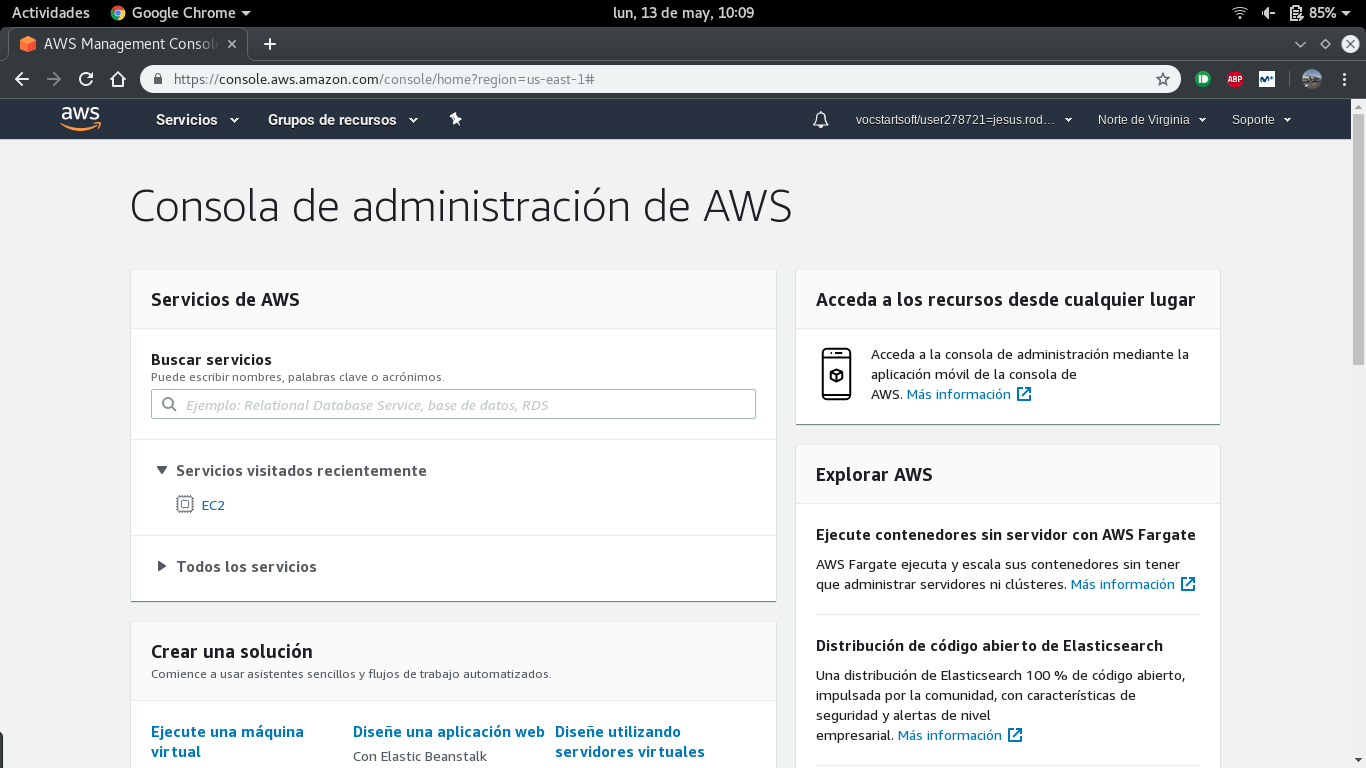
\includegraphics[scale=0.28]{ImagenesAWS/1.png}
		\caption{Consola de administración de AWS.}
		\label{Consola de administración de AWS}
	\end{figure}
	\item Seleccionamos ``Ejecute una máquina virtual''.
	\begin{figure}[h]
		\centering
		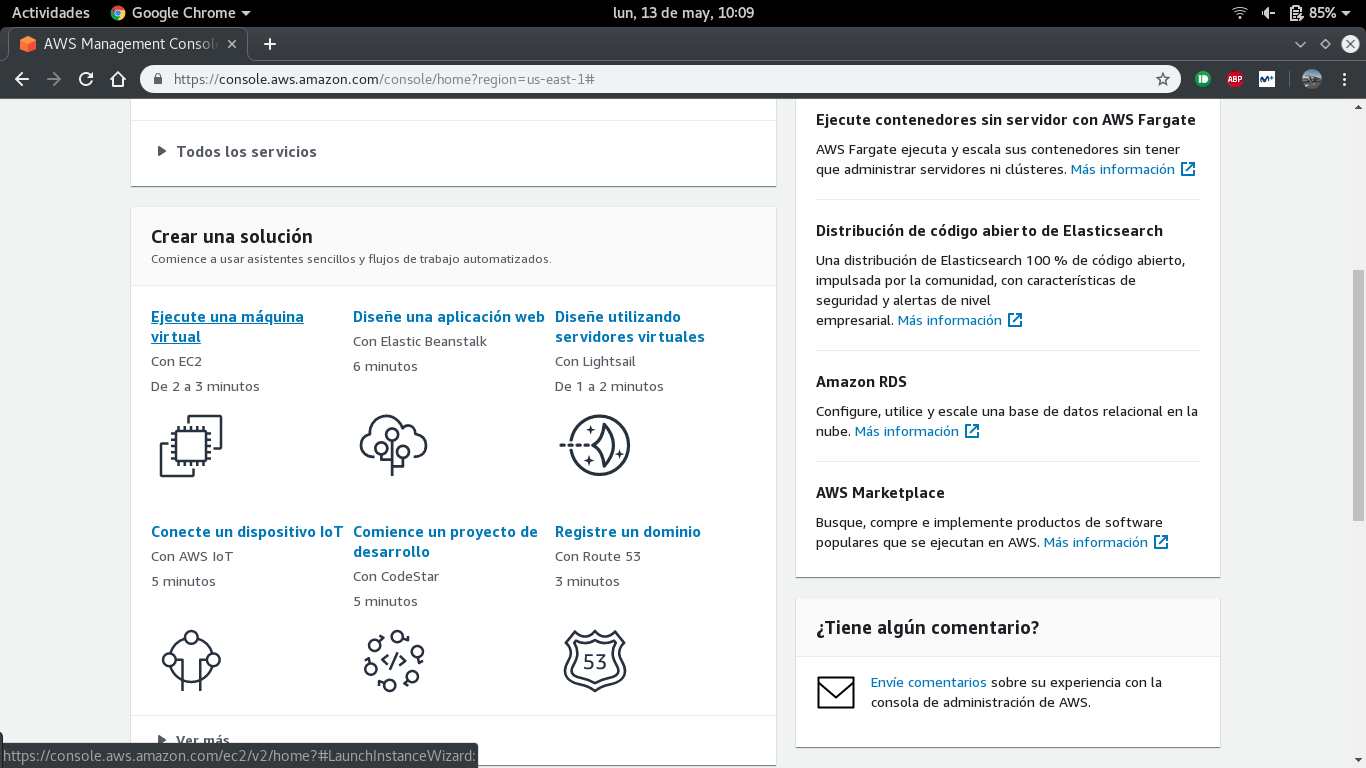
\includegraphics[scale=0.28]{ImagenesAWS/3.png}
		\caption{Selección de solución.}
		\label{Selección de solución}
	\end{figure}
\newpage
	\item Seleccionamos la AMI que deseemos, en nuestro caso será ``Ubuntu server 18.04 LTS (HVM), SSD Volume Type''.
	\begin{figure}[h]
		\centering
		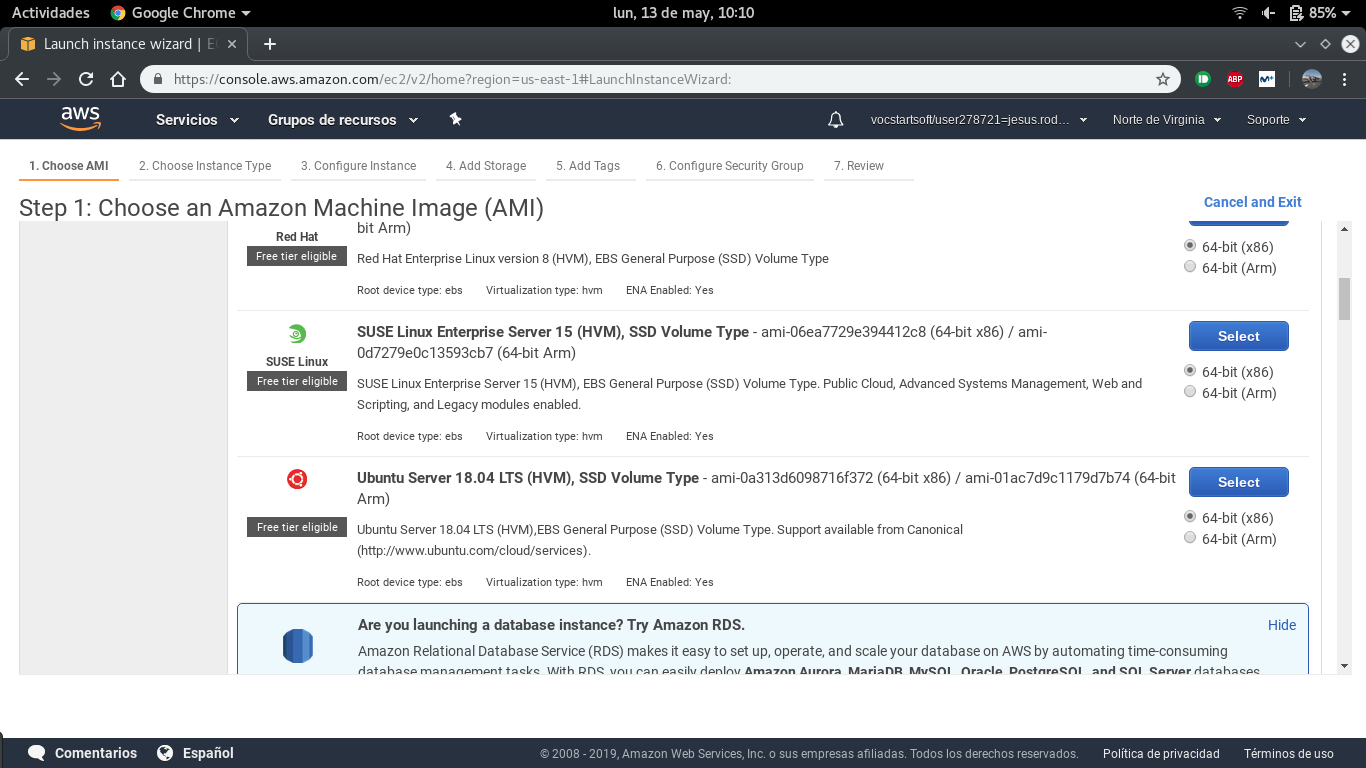
\includegraphics[scale=0.28]{ImagenesAWS/5.png}
		\caption{Selección de AMI.}
		\label{Selección de AMI}
	\end{figure}
	\item Seleccionamos el tipo de instancia que queremos:
	\begin{figure}[h]
		\centering
		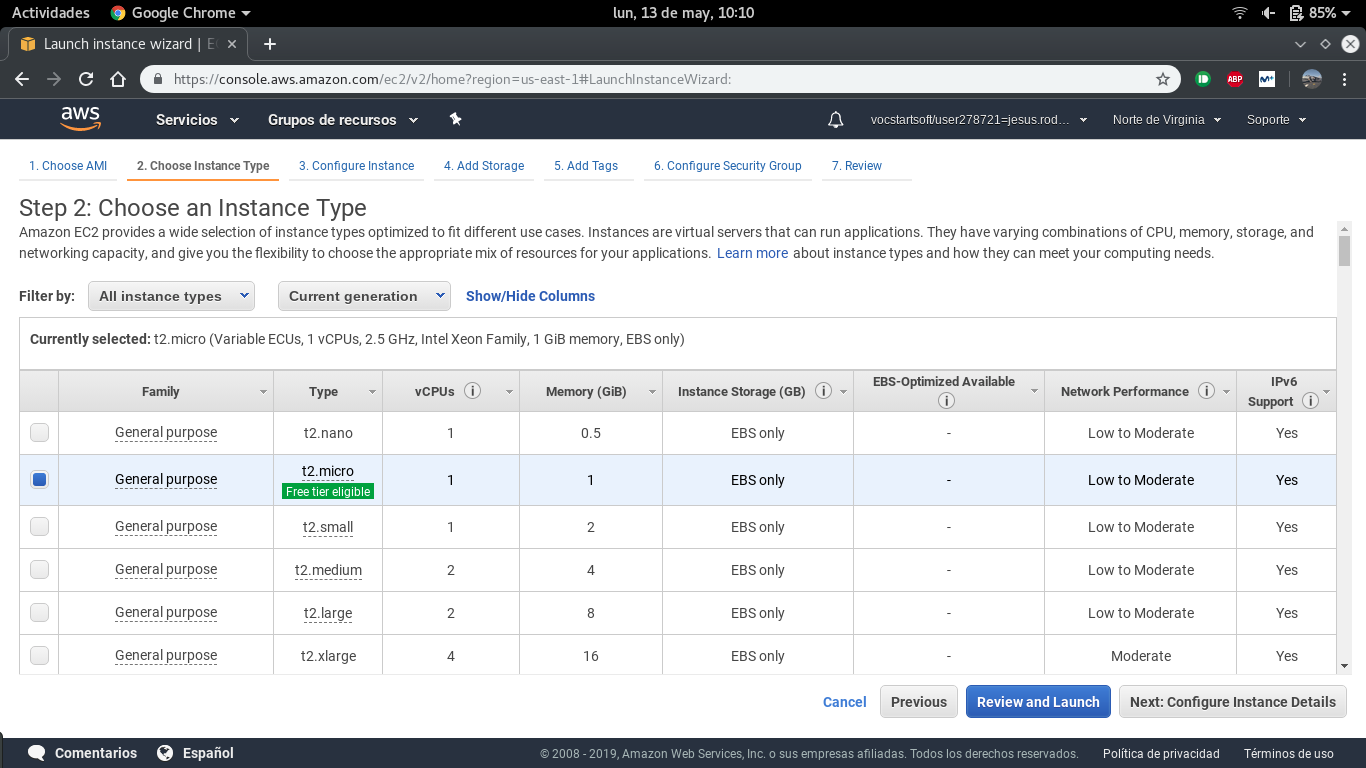
\includegraphics[scale=0.28]{ImagenesAWS/6.png}
		\caption{Selección de instancia.}
		\label{Selección de instancia}
	\end{figure}
\newpage
	\item Ahora debemos configurar los detalles que tendrá la instancia seleccionada:
	\begin{figure}[h]
		\centering
		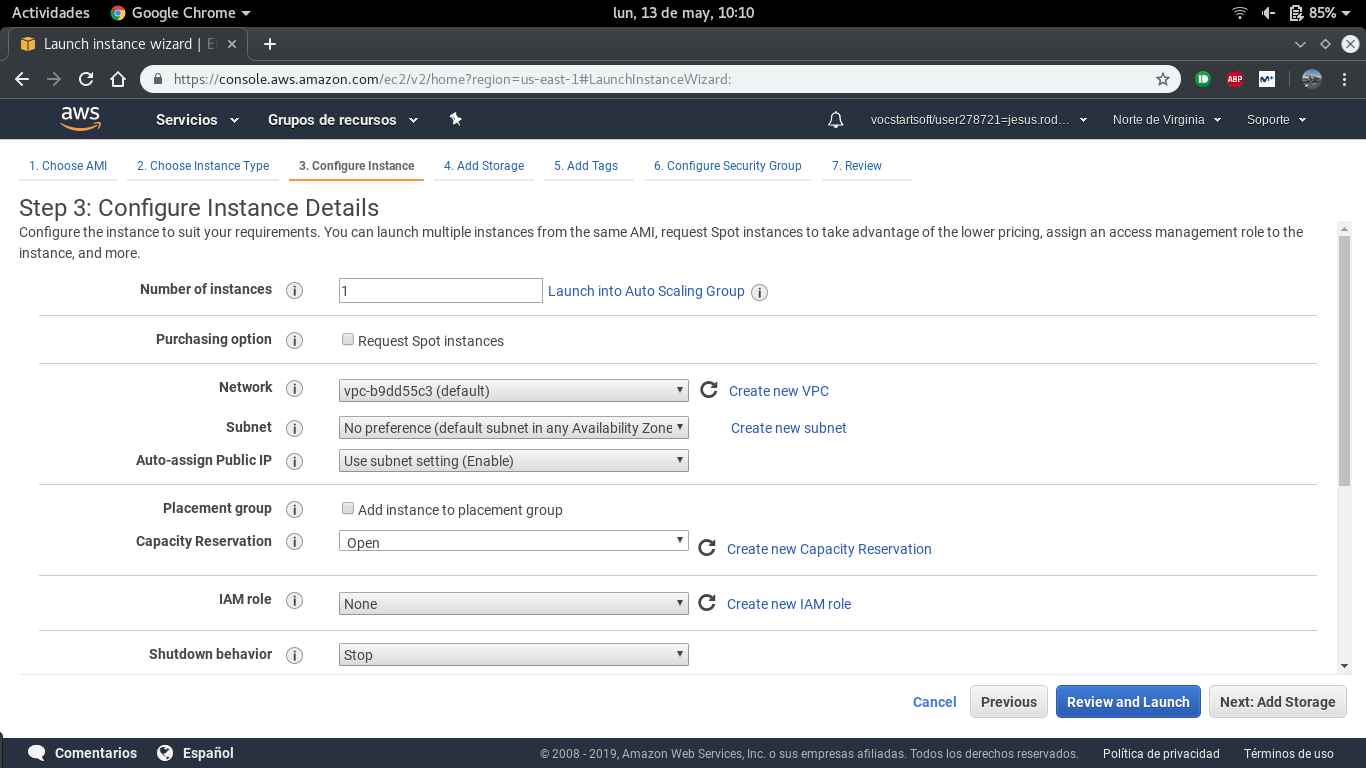
\includegraphics[scale=0.28]{ImagenesAWS/7.png}
		\caption{Configuración de la instancia.}
		\label{Configuración de la instancia}
	\end{figure}
	\item Seleccionamos el tamaño del almacenamiento y el tipo de disco duro:
	\begin{figure}[h]
		\centering
		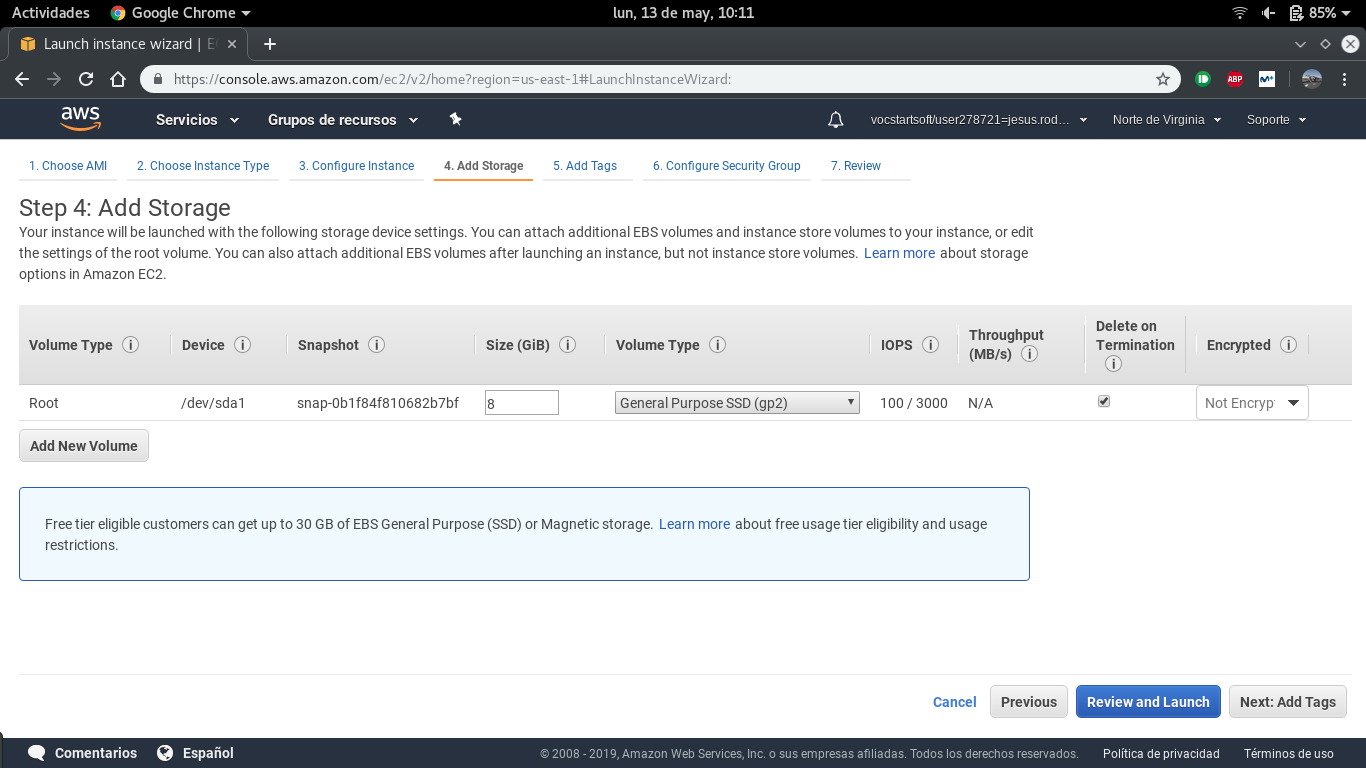
\includegraphics[scale=0.28]{ImagenesAWS/8.png}
		\caption{Selección de almacenamiento.}
		\label{Selección de almacenamiento}
	\end{figure}
\newpage
	\item Añadimos las etiquetas que deseemos:
	\begin{figure}[h]
		\centering
		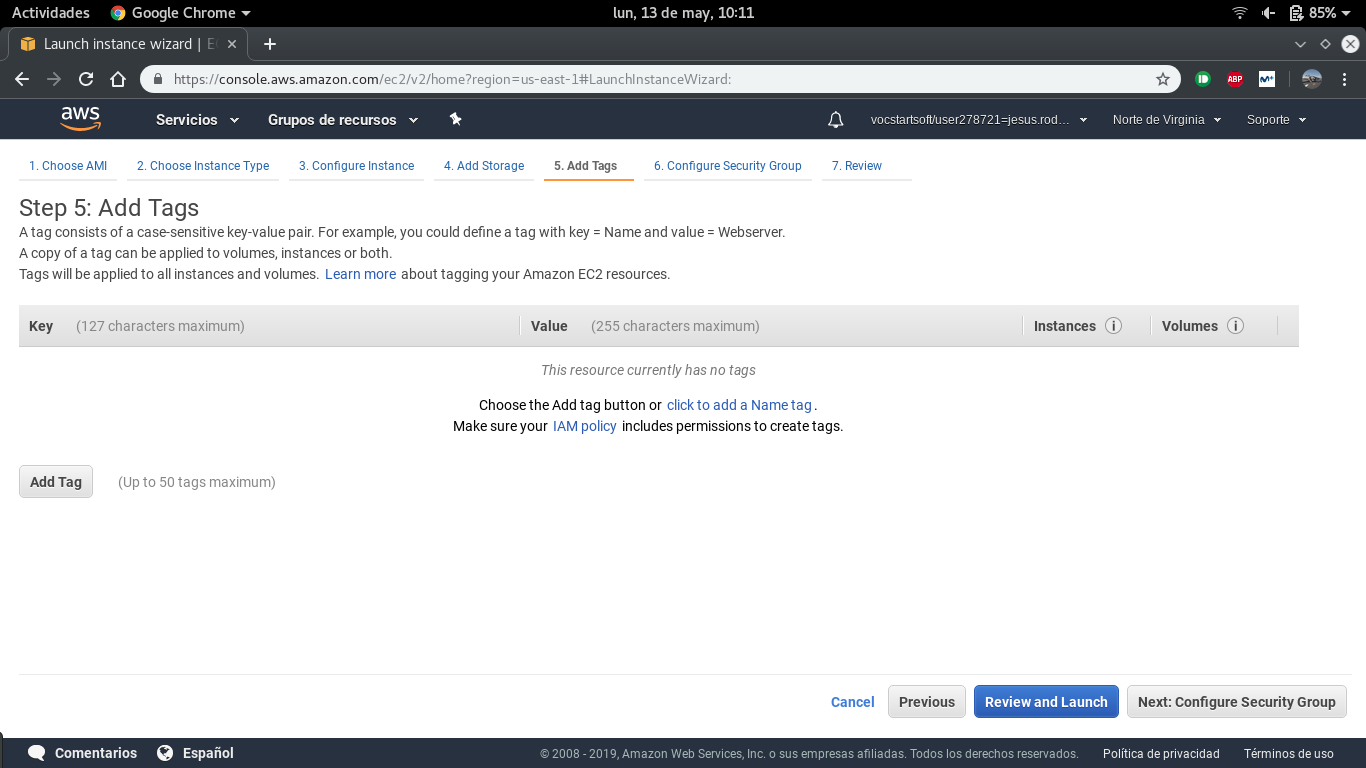
\includegraphics[scale=0.28]{ImagenesAWS/9.png}
		\caption{Añadimos las etiquetas.}
		\label{Añadimos las etiqutas}
	\end{figure}
	\item Configuramos las conexiones que vayamos a tener como el SSH:
	\begin{figure}[h]
		\centering
		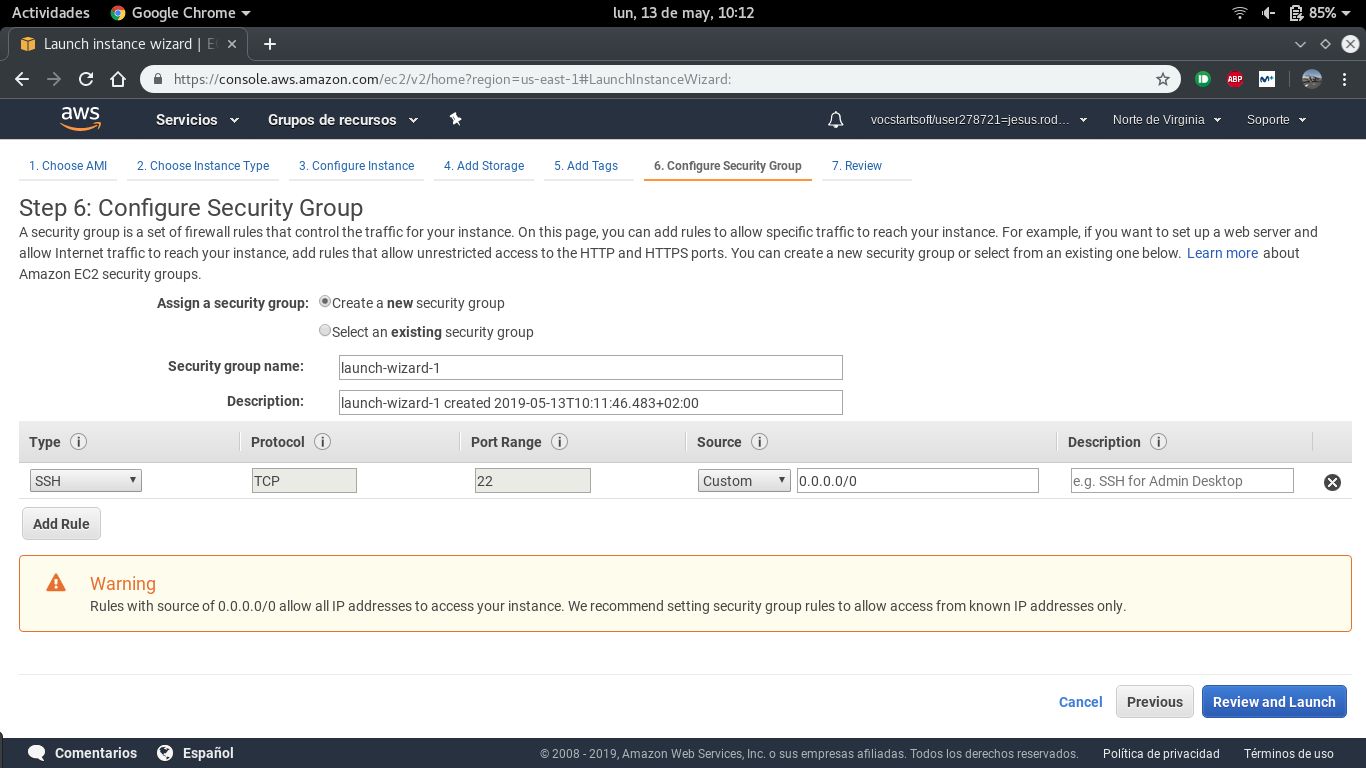
\includegraphics[scale=0.28]{ImagenesAWS/10.png}
		\caption{Configuración conexiones.}
		\label{Configuración de conexiones}
	\end{figure}
\newpage
	\item Finalmente, veremos una página con el resumen de las características que tendrá nuestra máquina:
	\begin{figure}[h]
		\centering
		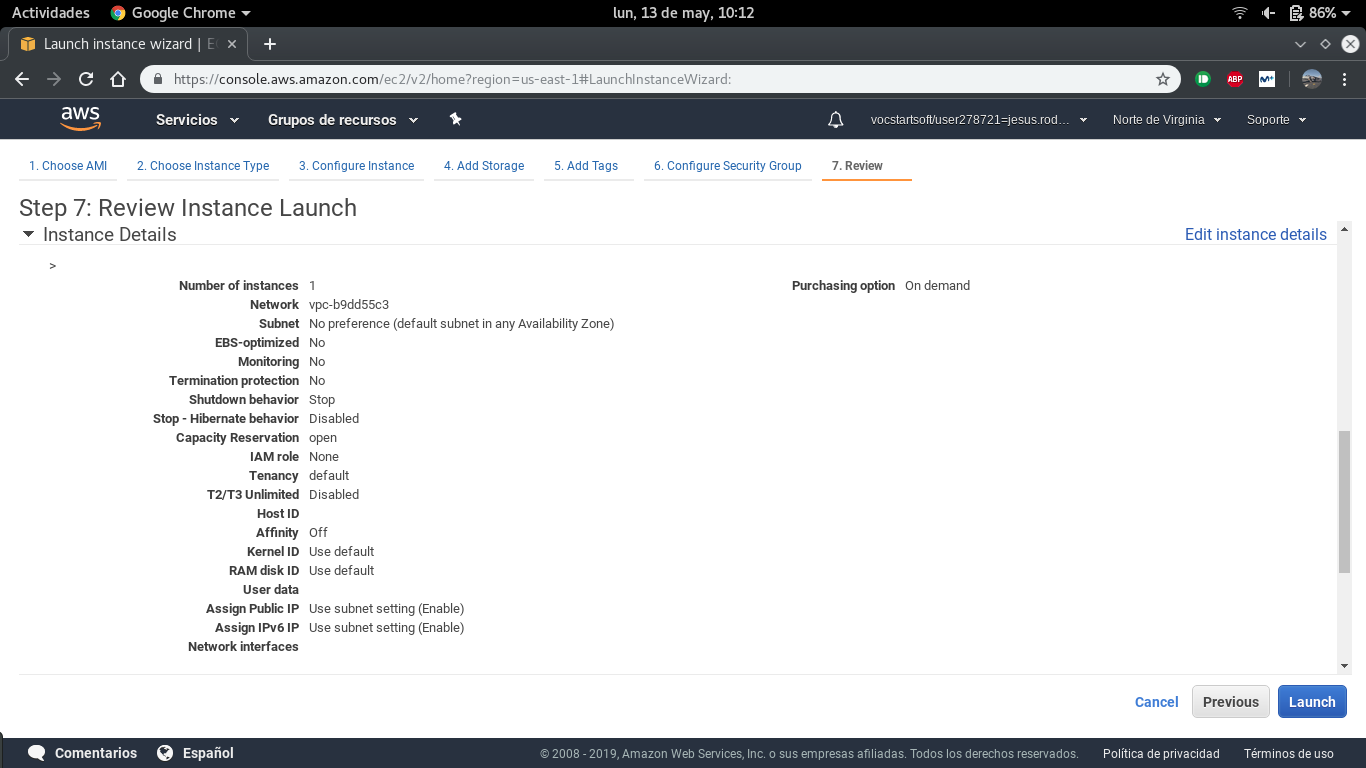
\includegraphics[scale=0.28]{ImagenesAWS/12.png}
		\caption{Resumen de la máquina.}
		\label{Resumen de la máquina}
	\end{figure}
	\item Cuando le damos a ``Launch'' nos saldrá la siguiente pestaña para generar y descargar la clave SSH:
	\begin{figure}[h]
		\centering
		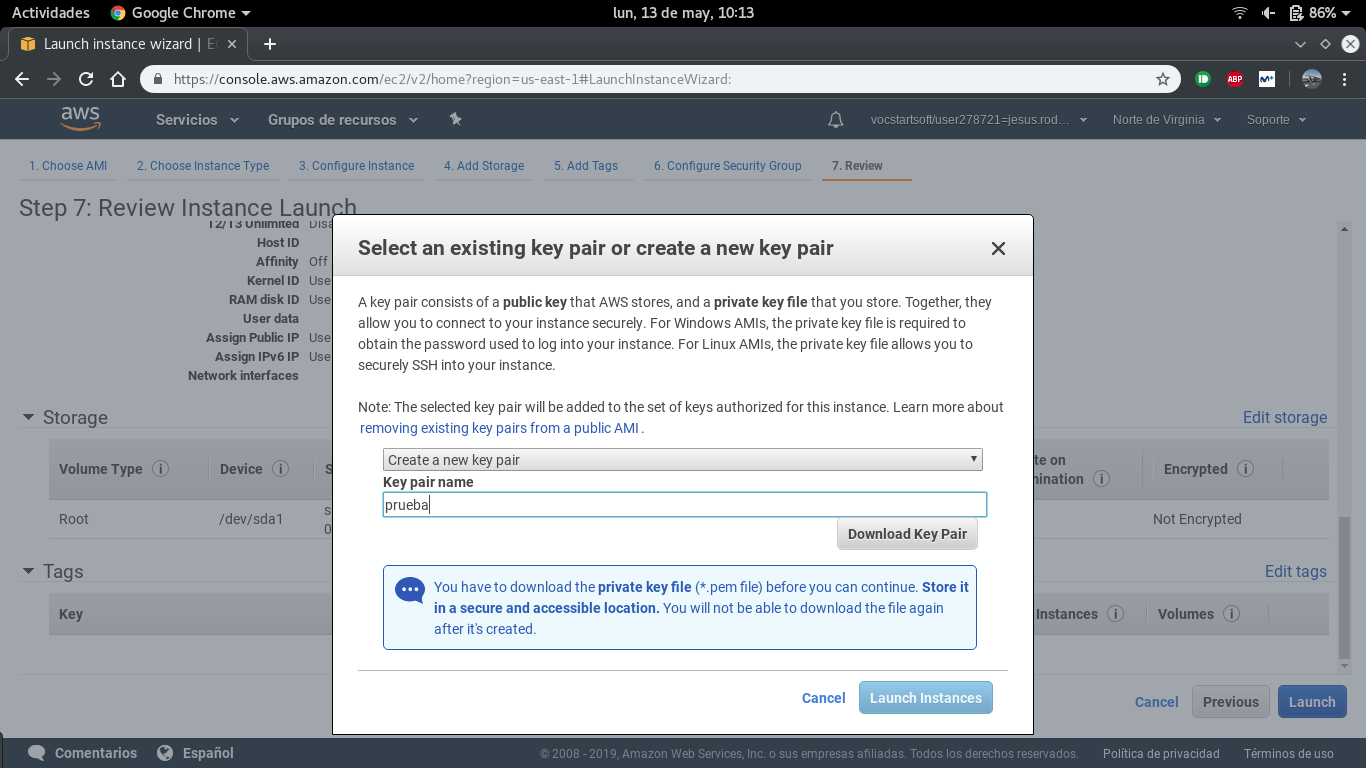
\includegraphics[scale=0.28]{ImagenesAWS/13.png}
		\caption{Creación de clave SSH.}
		\label{Creación de clave SSH}
	\end{figure}
\newpage
	\item Luego, en el apartado de ``Instancias'' de la consola de administración podremos ver nuestra máquina virtual ejecutándose:
	\begin{figure}[h]
		\centering
		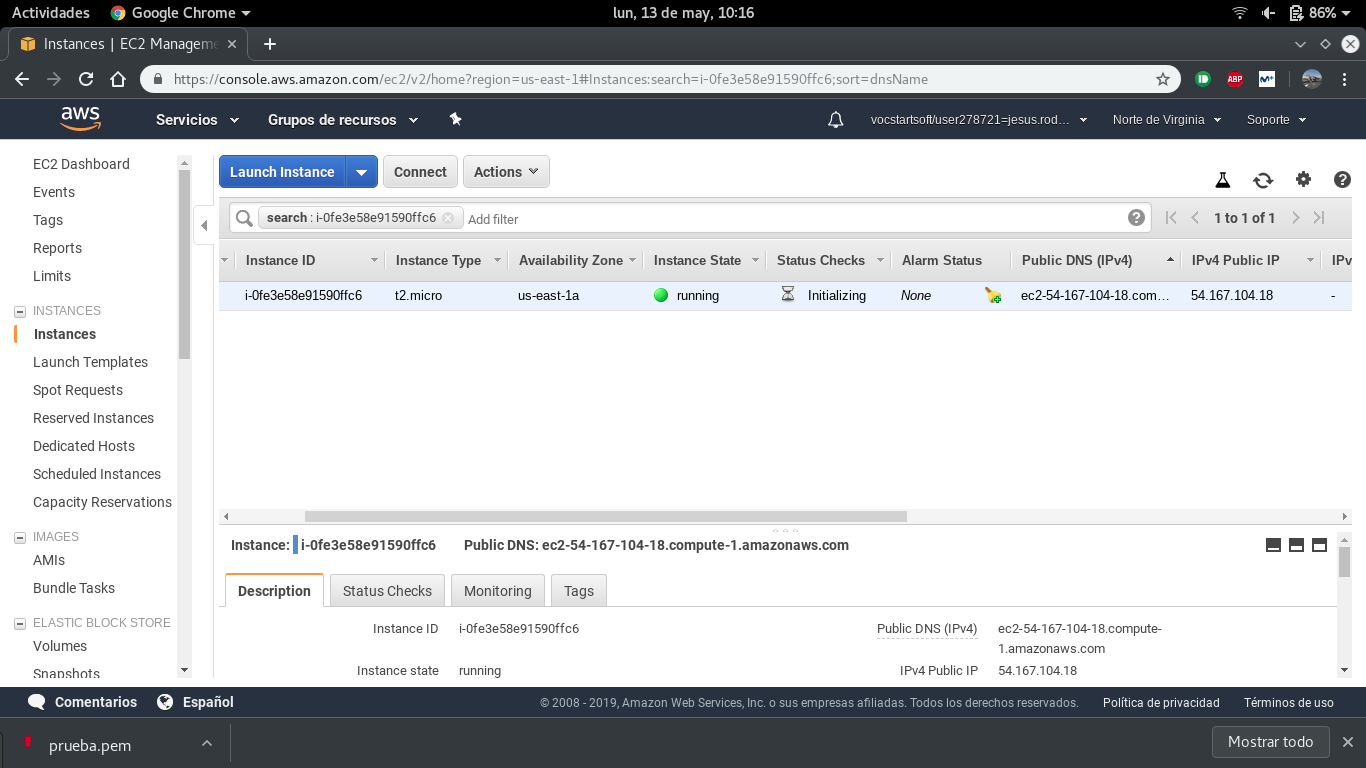
\includegraphics[scale=0.28]{ImagenesAWS/15.png}
		\caption{Máquina en ejecución.}
		\label{Máquina en ejecución}
	\end{figure}
	\item Para conectarnos a la máquina por SSH, debemos cambiar los permisos del fichero ``prueba.pem'' generado e introducir el siguiente comando:
	\begin{center}
		\texttt{ssh -i prueba.pem ubuntu@54.167.104.18}
	\end{center}
	\begin{figure}[h]
		\centering
		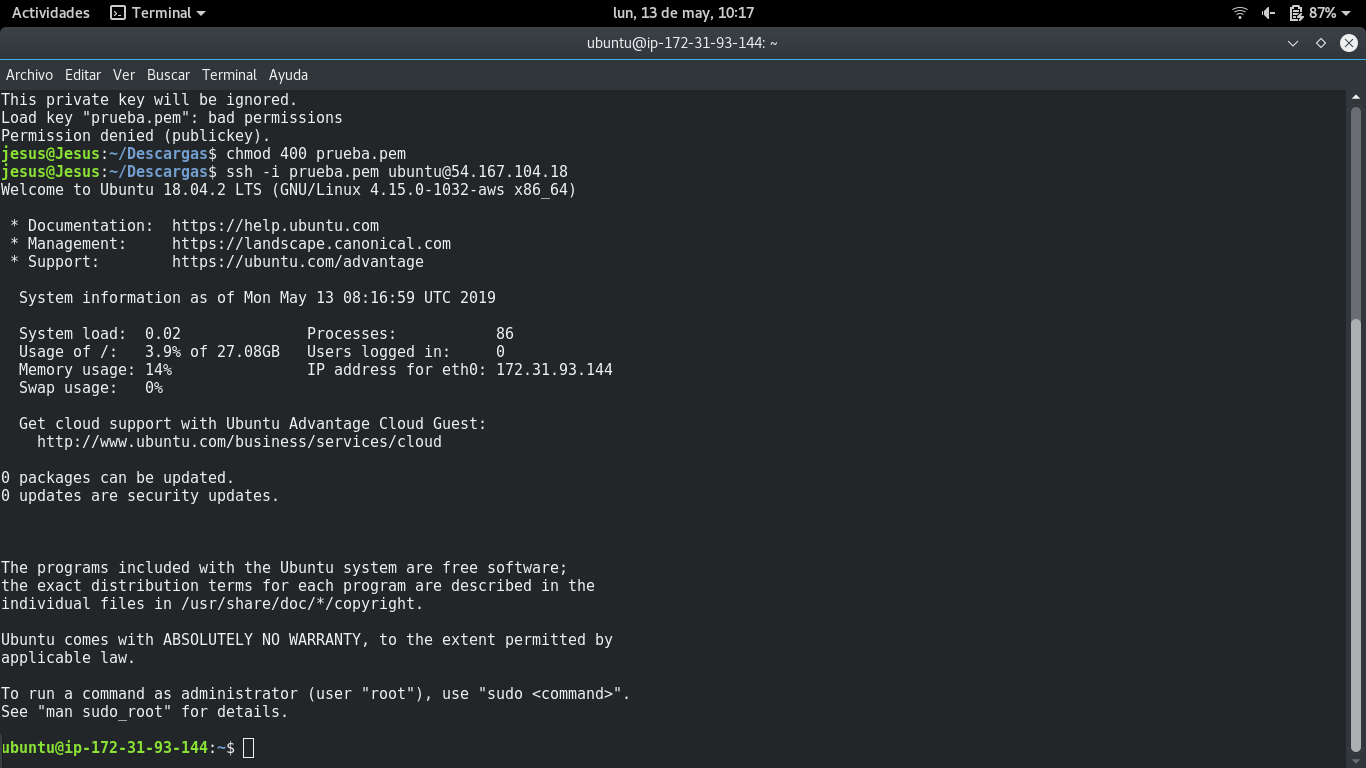
\includegraphics[scale=0.28]{ImagenesAWS/16.png}
		\caption{Conexión con la máquina virtual.}
		\label{Conexión con la máquina virtual}
	\end{figure}
\newpage
	\item Si lanzamos el comando: \texttt{cat /proc/cpuinfo}, podremos ver las características del procesador de nuestra máquina virtual.
	\begin{figure}[h]
		\centering
		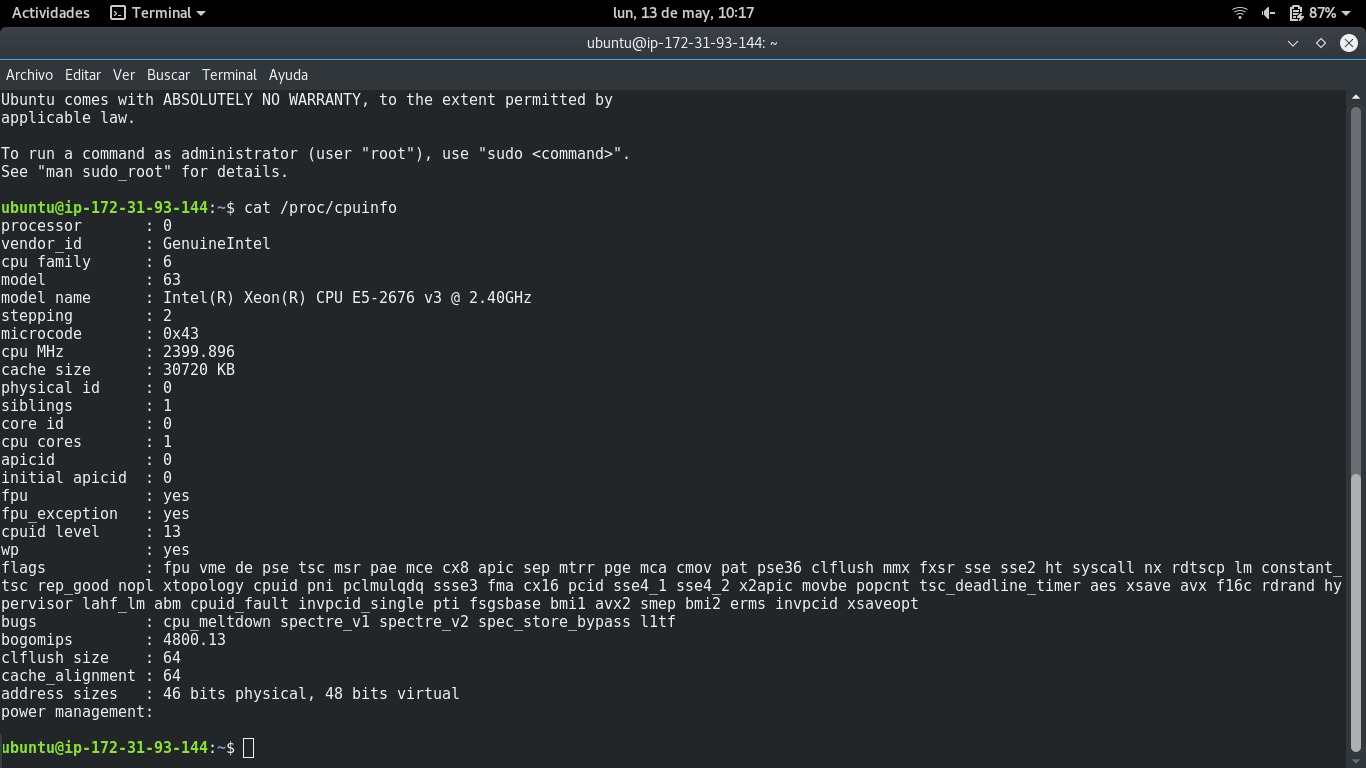
\includegraphics[scale=0.28]{ImagenesAWS/17.png}
		\caption{Información de la CPU de la máquina virtual.}
		\label{Información de la CPU de la máquina virtual}
	\end{figure}
	\item Para detener la ejecución de la máquina virtual, en la consola de administración, hacemos click derecho y seleccionamos ``Stop'' dentro de ``Instance State''. También es posible detener la máquina virtual con el comando \texttt{sudo shutdown now}.
	\begin{figure}[h]
		\centering
		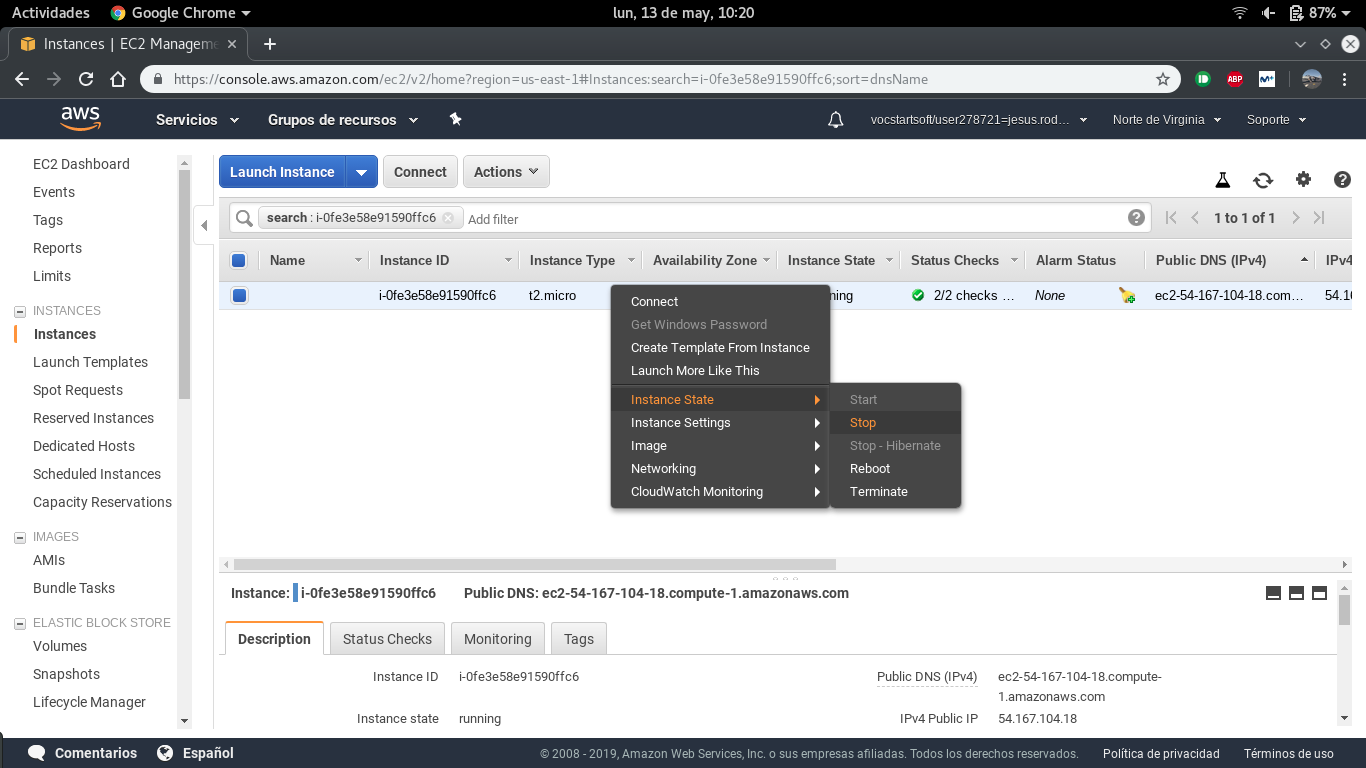
\includegraphics[scale=0.28]{ImagenesAWS/19.png}
		\caption{Detener la ejecución de la máquina virtual.}
		\label{Detener la ejecución de la máquina virtual}
	\end{figure}
\end{enumerate}

\newpage
\section{Creación de una máquina virtual en Azure}
La máquina B1ls de Azure seleccionada cuenta con las siguientes especificaciones técnicas:
\begin{itemize}
	\item Un vCPU.
	\item 0.5 GB de RAM.
	\item 4 GB de almacenamiento (HDD o SSD).
	\item 200 MB de transferencia.
\end{itemize}

Para crear el servicio, debemos seguir los siguientes pasos:
\begin{enumerate}
	\item Seleccionamos la opción ``máquinas virtuales'' del menú de la derecha:
	\begin{figure}[h]
		\centering
		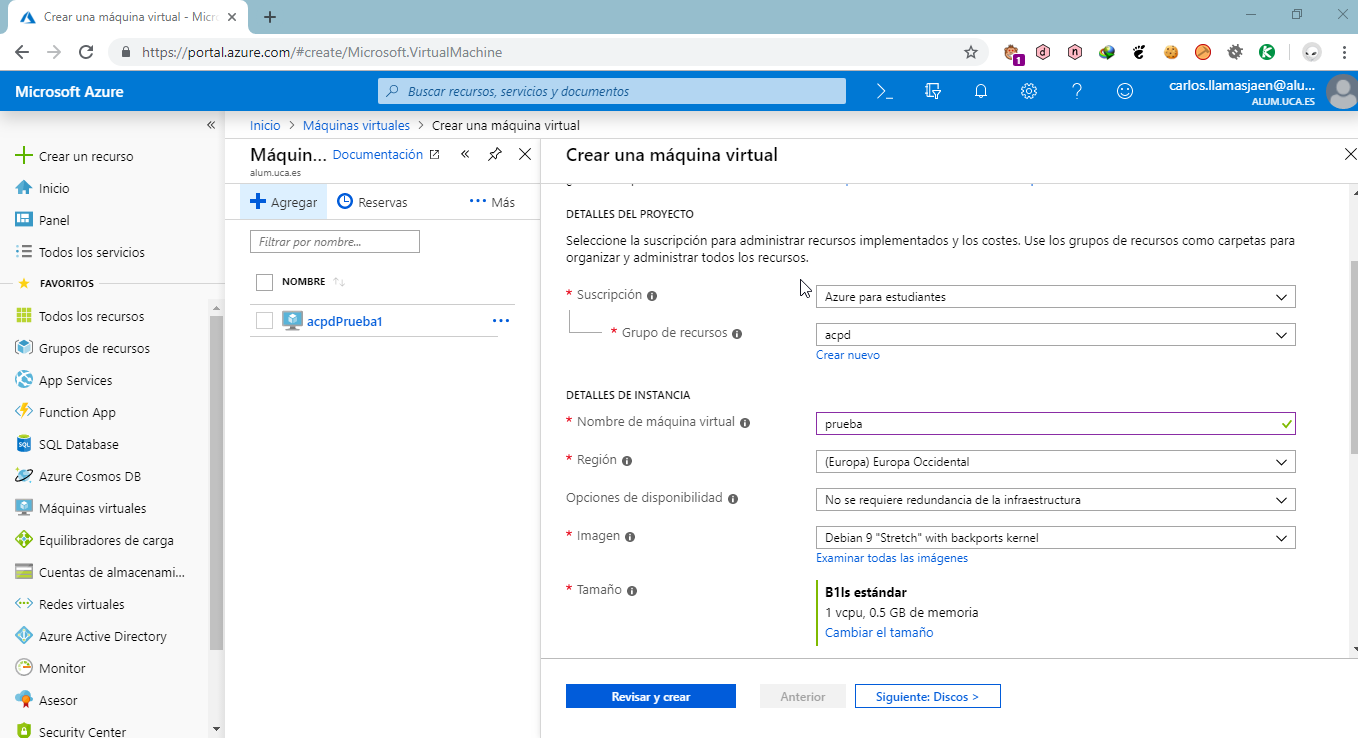
\includegraphics[scale=0.35]{ImagenesAzure/1.png}
		\caption{Crear máquina virtual.}
		\label{Crear máquina virtual}
	\end{figure}
\newpage
	\item Seleccionamos el tipo de instancia que queremos:
	\begin{figure}[h]
		\centering
		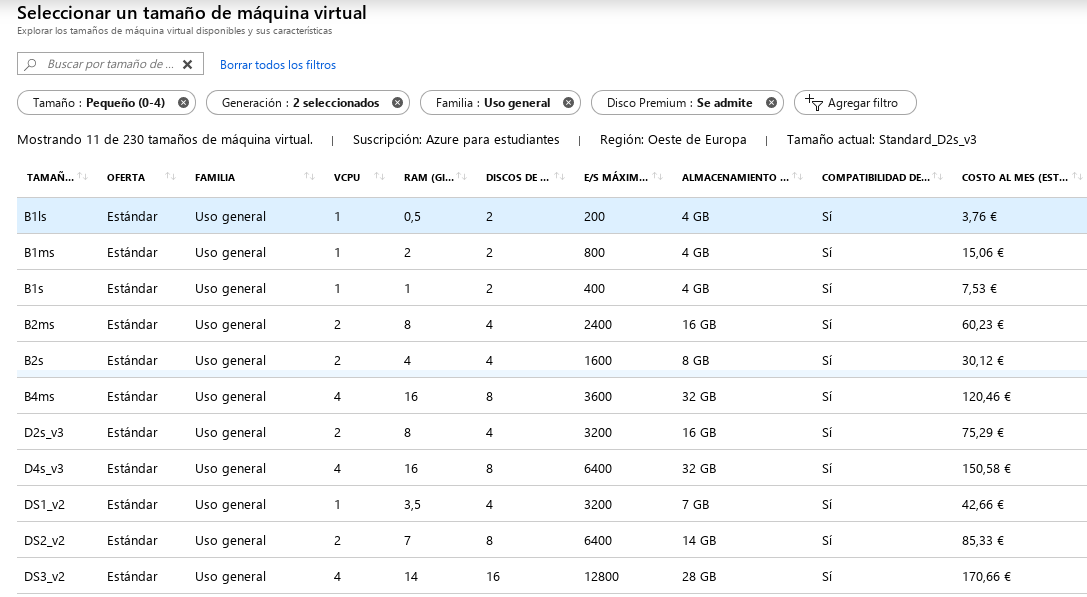
\includegraphics[scale=0.35]{ImagenesAzure/1medio.png}
		\caption{Selección de instancia.}
		\label{Selección de instancia2}
	\end{figure}
	\item Establecemos el tipo de autenticación por SSH y añadimos la clave pública:
	\begin{figure}[h]
		\centering
		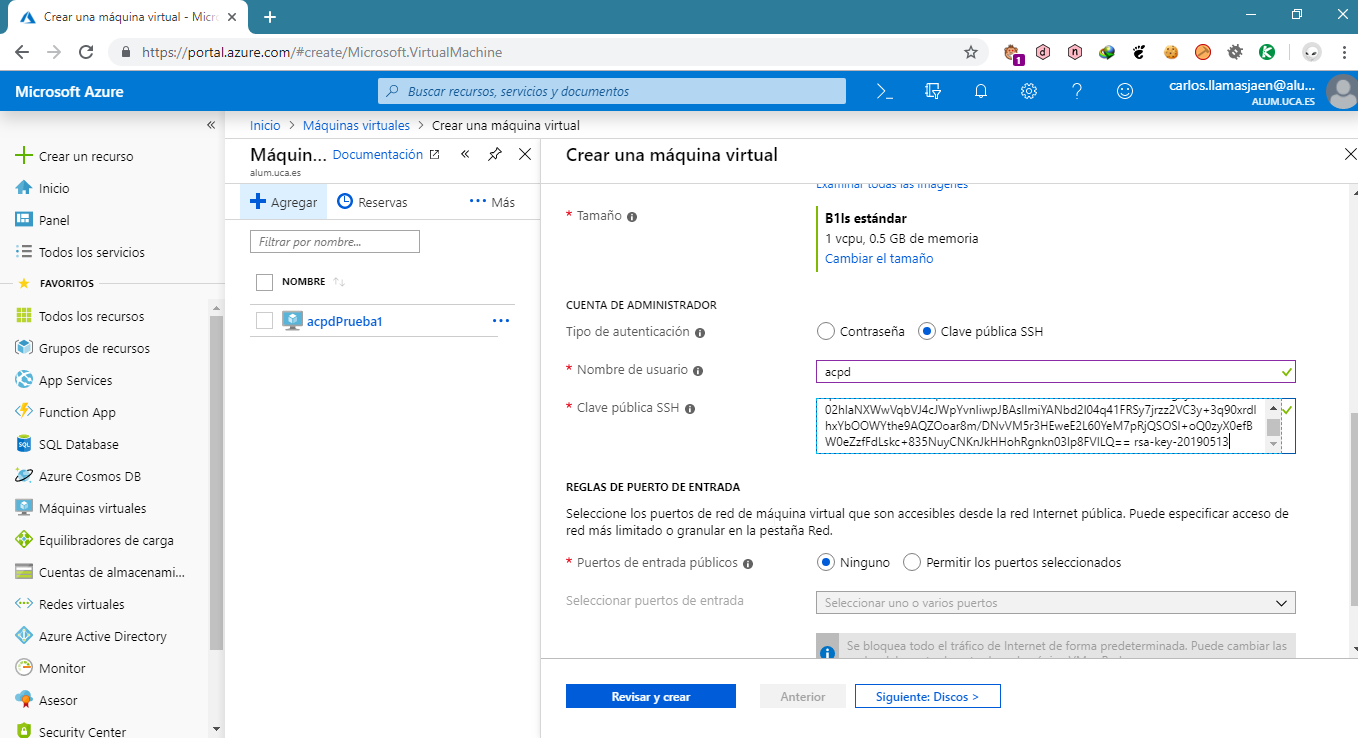
\includegraphics[scale=0.35]{ImagenesAzure/2.png}
		\caption{Establecer autenticación por SSH.}
		\label{Establecer autenticación por SSH}
	\end{figure}
\newpage
	\item Seleccionamos el tamaño de almacenamiento:
	\begin{figure}[h]
		\centering
		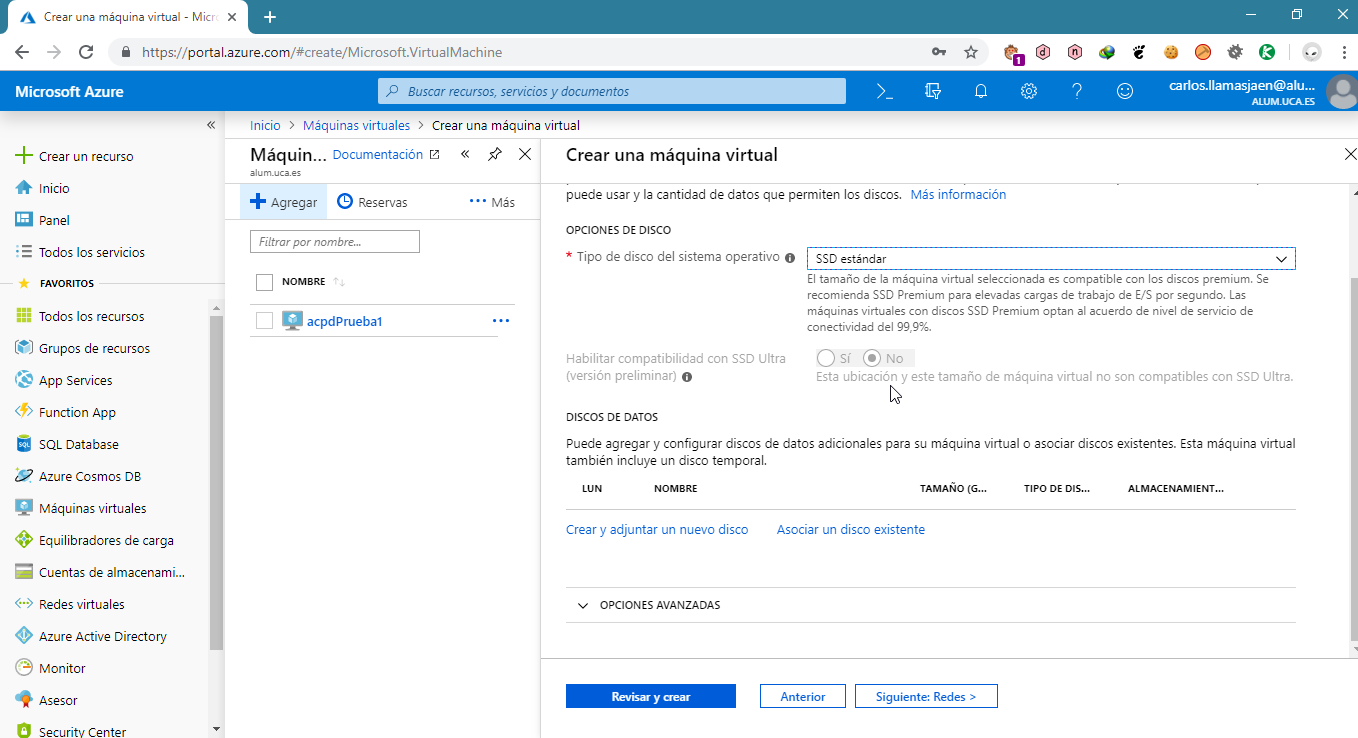
\includegraphics[scale=0.35]{ImagenesAzure/3.png}
		\caption{Selección de almacenamiento.}
		\label{Selección de almacenamiento2}
	\end{figure}
	\item Configuramos las redes virtuales:
	\begin{figure}[h]
		\centering
		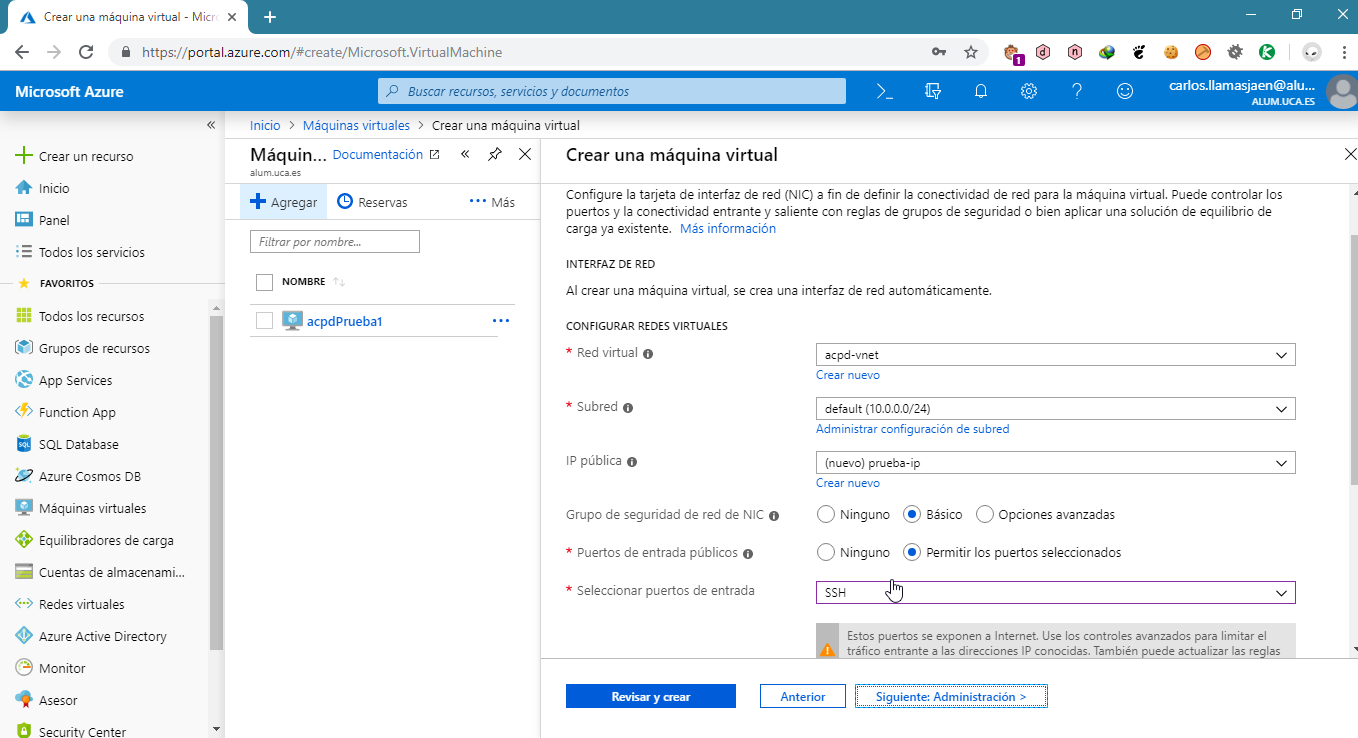
\includegraphics[scale=0.35]{ImagenesAzure/4.png}
		\caption{Configuración de redes virtuales.}
		\label{Configuración de redes virtuales}
	\end{figure}
\newpage
	\item Seleccionamos los puertos de entrada y si queremos equilibrio de carga:
	\begin{figure}[h]
		\centering
		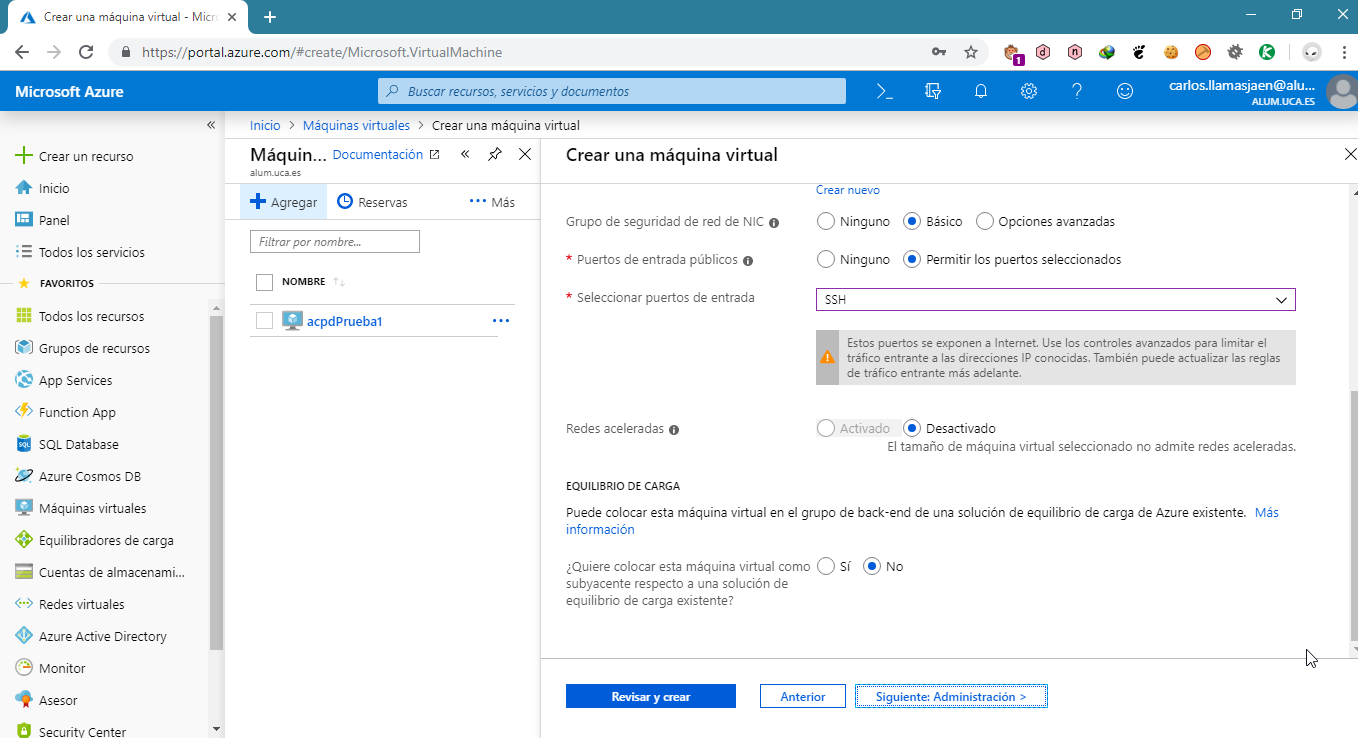
\includegraphics[scale=0.35]{ImagenesAzure/5.png}
		\caption{Selección de entrada y equilibrio de carga.}
		\label{Selección de entrada y equilibrio de carga}
	\end{figure}
	\item Añadimos la configuración de seguridad:
	\begin{figure}[h]
		\centering
		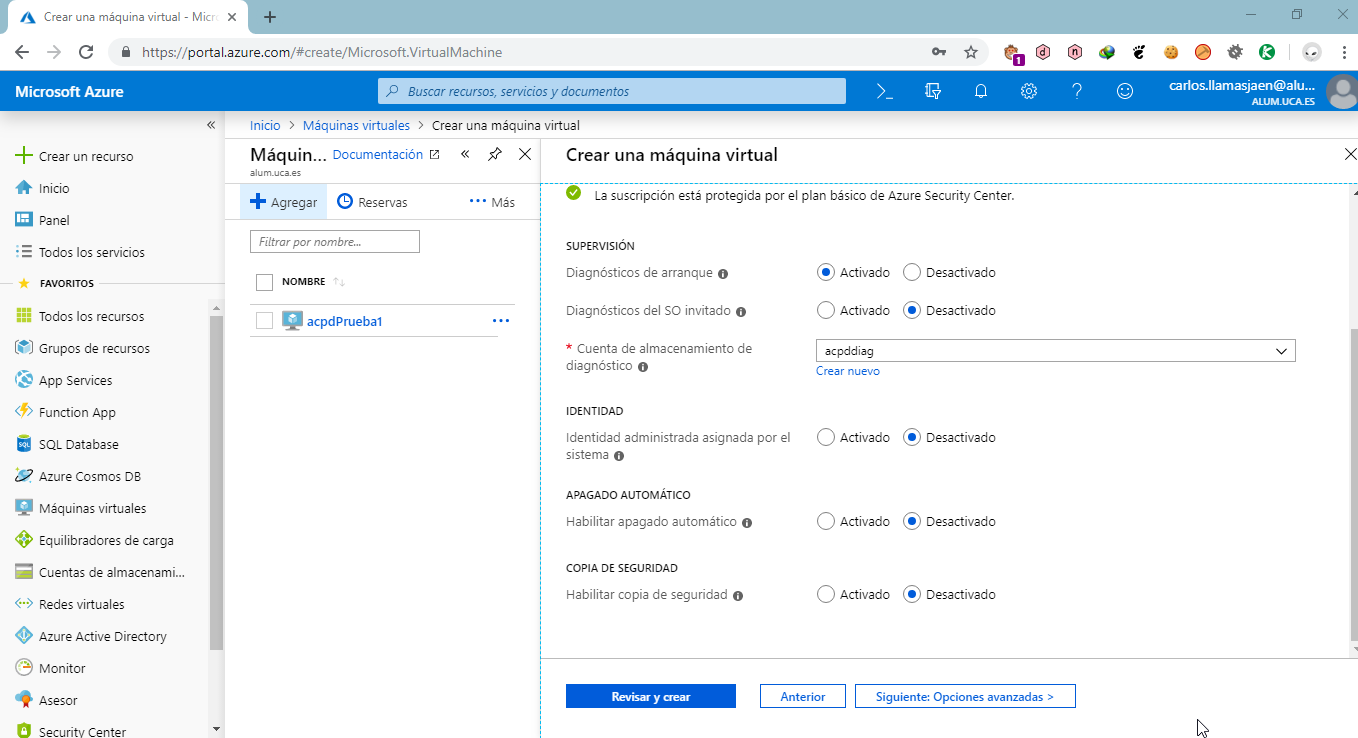
\includegraphics[scale=0.35]{ImagenesAzure/7.png}
		\caption{Configuración de seguridad.}
		\label{Configuración de seguridad}
	\end{figure}
\newpage
	\item Luego veremos las extensiones dentro de las opciones avanzadas:
	\begin{figure}[h]
		\centering
		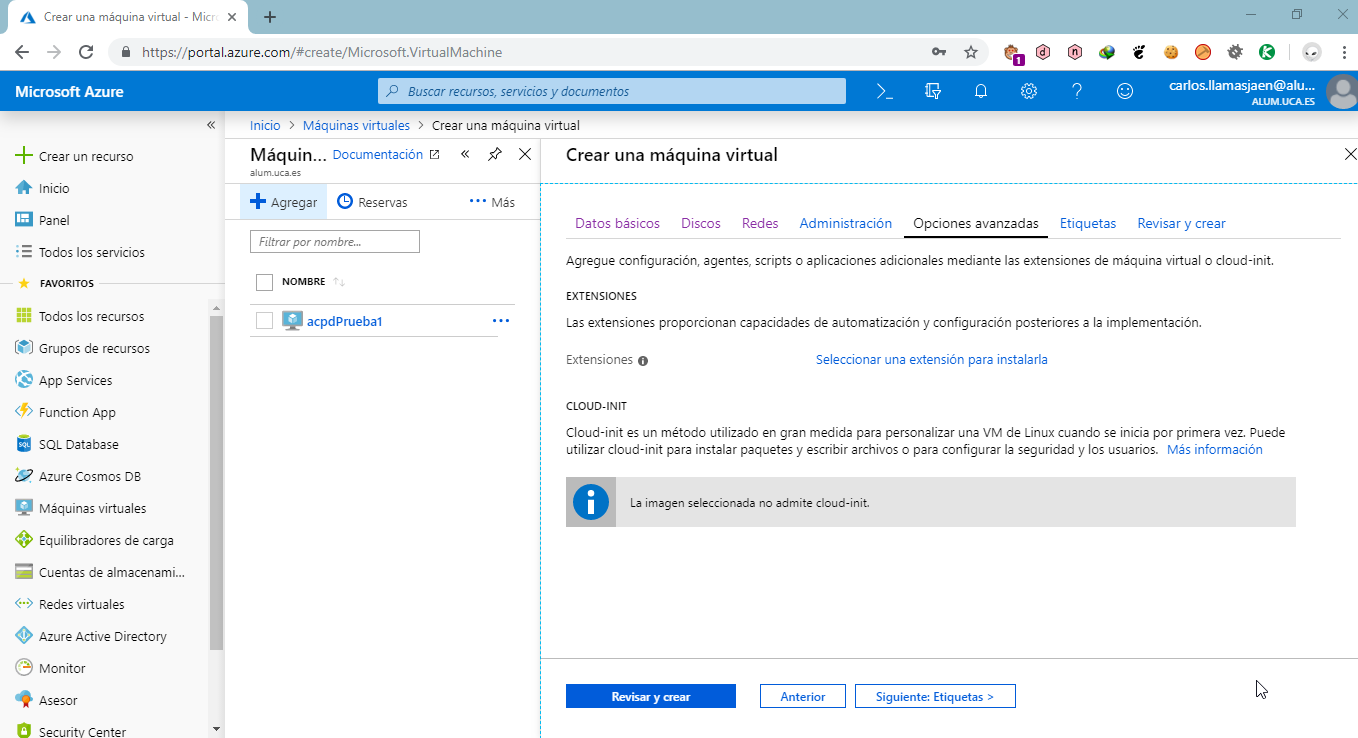
\includegraphics[scale=0.35]{ImagenesAzure/8.png}
		\caption{Opciones avanzadas.}
		\label{Opciones avanzadas}
	\end{figure}
	\item Añadimos las etiquetas que deseemos:
	\begin{figure}[h]
		\centering
		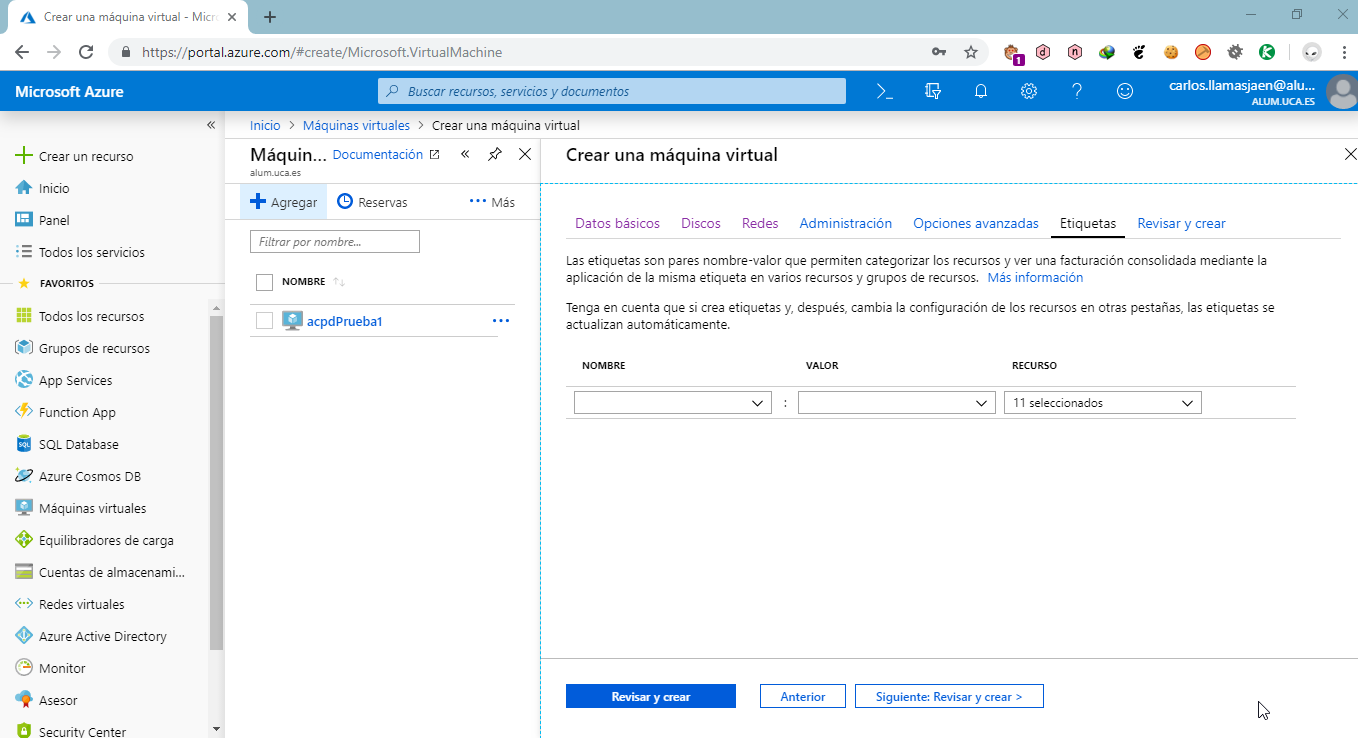
\includegraphics[scale=0.35]{ImagenesAzure/9.png}
		\caption{Añadimos las etiquetas.}
		\label{Añadimos las etiqutas2}
	\end{figure}
\newpage
	\item Finalmente, revisamos la configuración y creamos la máquina virtual:
	\begin{figure}[h]
		\centering
		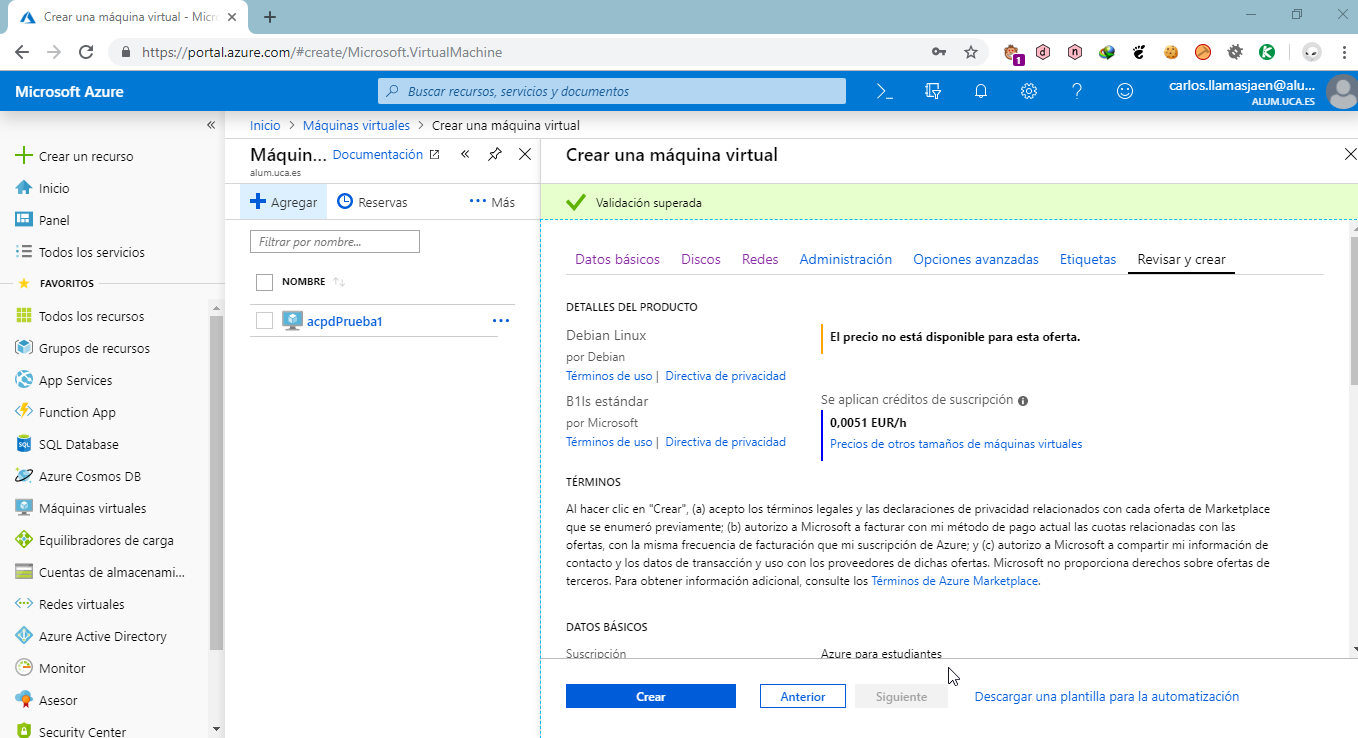
\includegraphics[scale=0.35]{ImagenesAzure/10.png}
		\caption{Revisión de la configuración.}
		\label{Revisión de la configuración}
	\end{figure}
	\item Para conectarnos, lo haremos por ssh a la IP indicada y para ver las especificaciones de la CPU de la máquina virtual usaremos el comando \texttt{cat /proc/cpuinfo}:
	\begin{figure}[h]
		\centering
		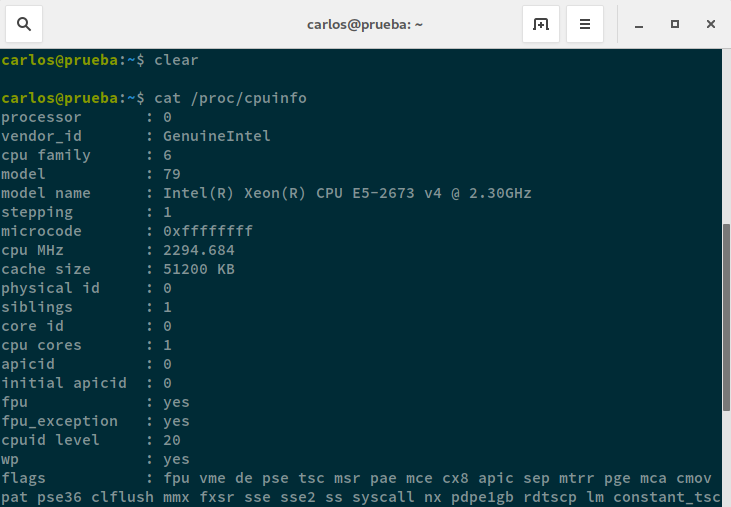
\includegraphics[scale=0.45]{ImagenesAzure/cpuinfo.png}
		\caption{Información del procesador.}
		\label{Información del procesador}
	\end{figure}
\end{enumerate}